\subsection{Lora}
\subsubsection{Integrating single LoRA component to SAM}
This section presents the performance and parameter efficiency of integrating LoRA into the SAM image encoder. Following the optimal hyperparameters identified in the preliminary results, all experiments were conducted using a learning rate of $1e^{-4}$. The evaluation compares vit\_l and vit\_b backbones across ranks 32 and 64 to determine the impact of model capacity and adaptation rank on segmentation accuracy.

\begin{table}[h]
\centering
\begin{tabular}{lccc}
\hline
Backbone & Rank & IOU AR & IOU TC \\
\hline
vit\_l & 64 & 0.4136 & 0.6005 \\
vit\_l & 32 & 0.4060 & 0.6009 \\
vit\_b & 64 & 0.4387 & 0.6201 \\
vit\_b & 32 & 0.4222 & 0.6020 \\
\hline
\end{tabular}
\caption{LoRA Performance Comparison}
\label{tab:lora_performance}
\end{table}



Table \ref{tab:lora_performance} details the IOU scores for AR and TC. The vit\_b backbone consistently achieves higher accuracy than vit\_l across all configurations. At rank 64, vit\_b reaches an IOU of 0.4387 for AR and 0.6201 for TC, while vit\_l achieves 0.4136 and 0.6005, respectively. For both architectures, increasing the rank from 32 to 64 results in improved IOU scores, particularly for AR detection.

The parameter distribution and training overhead are shown in Table \ref{tab:lora_params_final}. The vit\_l configuration with rank 64 utilizes 14.41M trainable parameters, which represents 4.41\% of the total model. In comparison, the vit\_b configuration with rank 64 uses 10.48M trainable parameters, accounting for 10.06\% of its total architecture. While vit\_l has a larger total parameter count due to its frozen backbone, vit\_b requires fewer absolute trainable parameters and provides superior IOU results.


\begin{table}[h]
\centering
\begin{tabular}{lcccccccc}
\hline
Backbone & Rank & Adapter & Decoder & LoRA & Train & Frozen & Total & \% Train \\
\hline
vit\_l & 64 & 5.2K & 8.12M & 6.29M & 14.41M & 312.34M & 326.75M & 4.41\% \\
vit\_l & 32 & 5.2K & 8.12M & 3.14M & 11.26M & 312.34M & 323.61M & 3.48\% \\
vit\_b & 64 & 5.2K & 8.12M & 2.35M & 10.48M & 93.73M & 104.21M & 10.06\% \\
vit\_b & 32 & 5.2K & 8.12M & 3.14M & 9.30M & 93.73M & 103.03M & 9.03\% \\
\hline
\end{tabular}
\caption{Detailed Parameter Breakdown for LoRA-Adapted SAM}
\label{tab:lora_params_final}
\end{table}

The training dynamics illustrated in Figure \ref{fig:iou_lora_single} provide insights into model generalization and overfitting. While AR validation curves show steady improvement or stabilization, TC curves exhibit significant fluctuations and a decline in performance after an early peak.

For both vit\_b and vit\_l backbones, the TC validation IOU reaches its maximum within the first 10 to 15 epochs before degrading. This behavior suggests the models begin to memorize specific noise in TC training samples rather than learning generalized features. This trend is especially pronounced in vit\_l configurations, which fail to maintain a stable validation IOU despite their larger capacity. The instability in TC curves suggests that its smaller, localized structures are more susceptible to overfitting during LoRA adaptation.

\begin{figure}[!h]
    \centering
    \begin{minipage}[b]{0.45\textwidth}
        \centering
        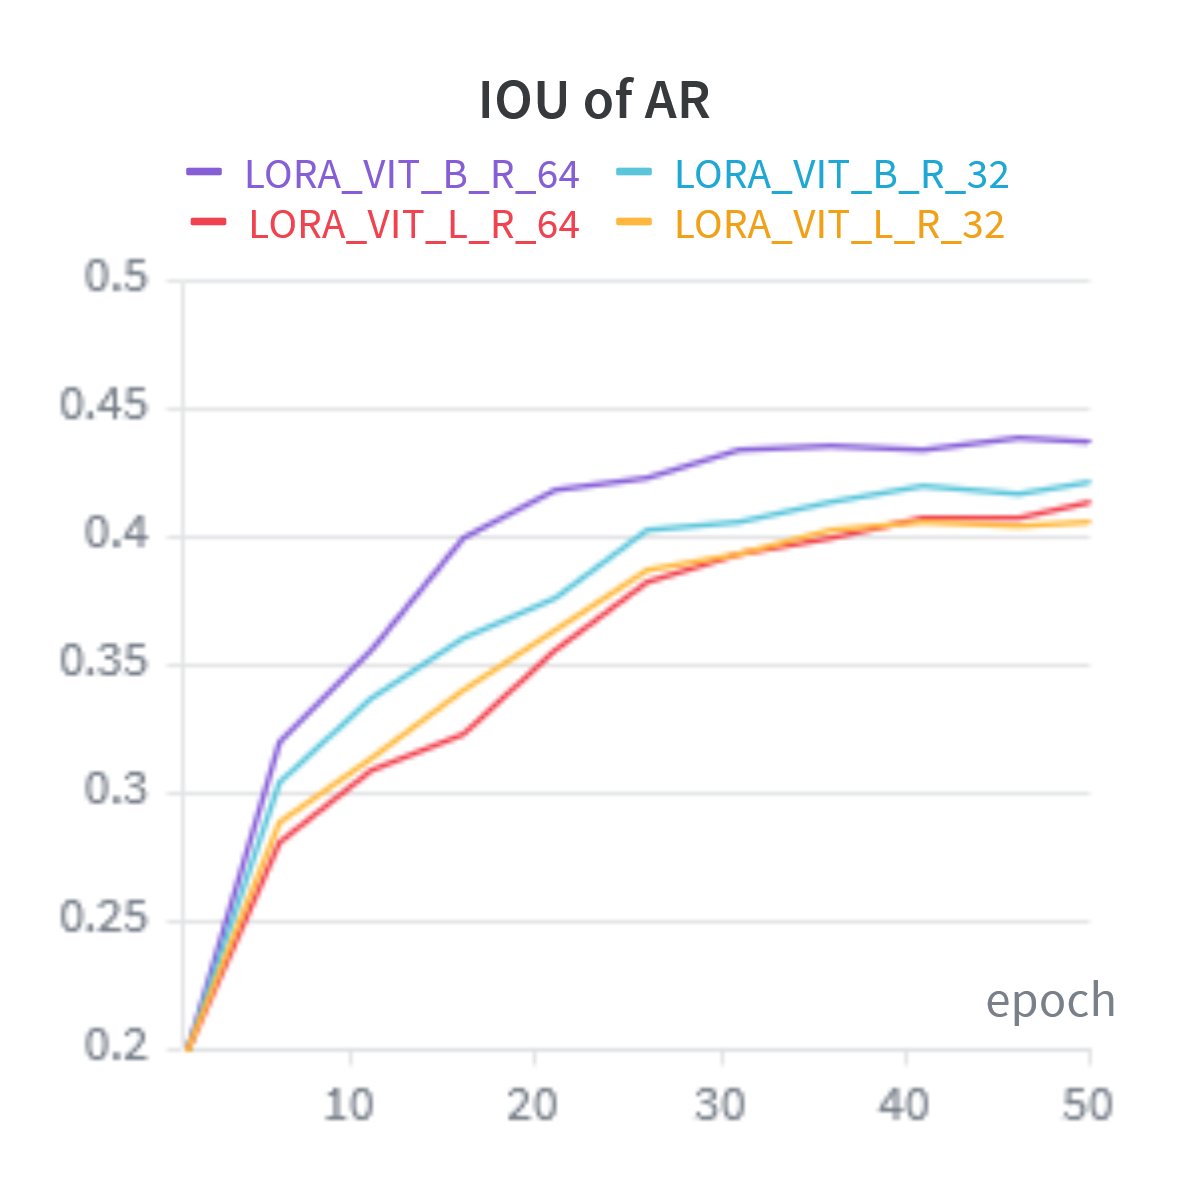
\includegraphics[width=\textwidth]{graphics/result/LORA_SING_AR.png}
        \caption{AR Validation IOU}
    \end{minipage}
    \hfill
    \begin{minipage}[b]{0.45\textwidth}
        \centering
        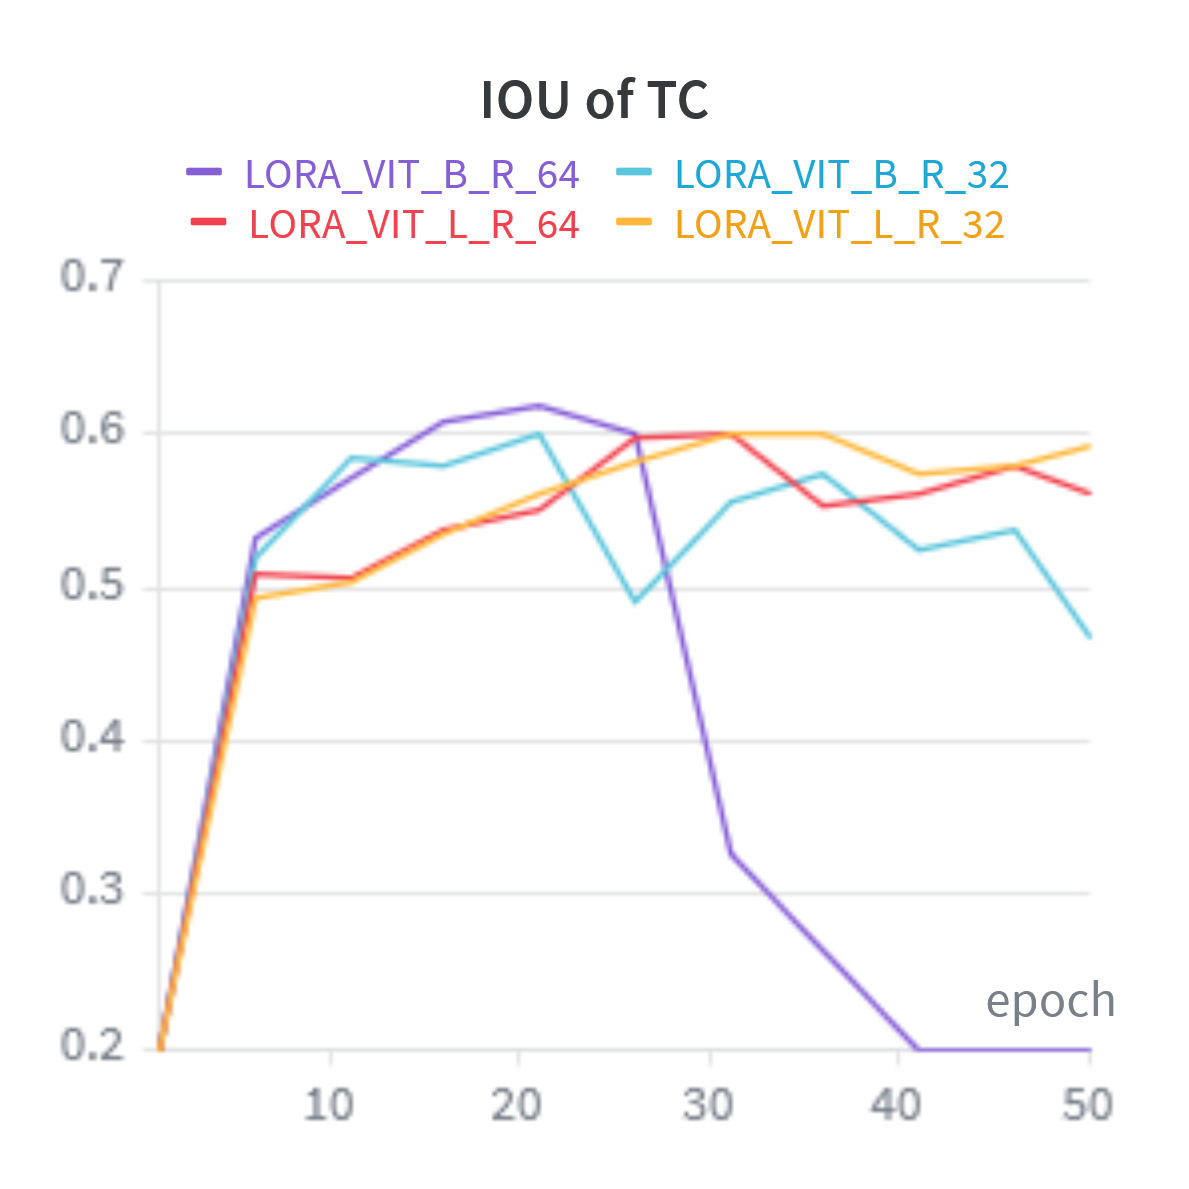
\includegraphics[width=\textwidth]{graphics/result/LORA_SINGLE_TC.png}
        \caption{TC Validation IOU}
    \end{minipage}
    \caption{Validation IOU curves for AR and TC during training}
    \label{fig:iou_lora_single}
\end{figure}
\subsubsection{Integrating single LoRA component to SAM [WITH AUGMENTATION]}
To address TC overfitting, we investigated data augmentation using Horizontal Flip, Vertical Flip, and Random Horizontal Roll ($p=0.5$, shift\_limit$=0.5$). We hypothesized these geometric transforms would be counterproductive as ClimateNet relies on global spatial compositions where geographic orientation is critical. The results in Figure \ref{fig:lora_augmentation} confirm this; while augmentation narrowed the training-validation gap, it hindered effective generalization, causing a sharp mIoU decline for both AR and TC compared to the non-augmented baseline.
\begin{figure}[!h]
    \centering
    \begin{minipage}[b]{0.8\textwidth}
        \centering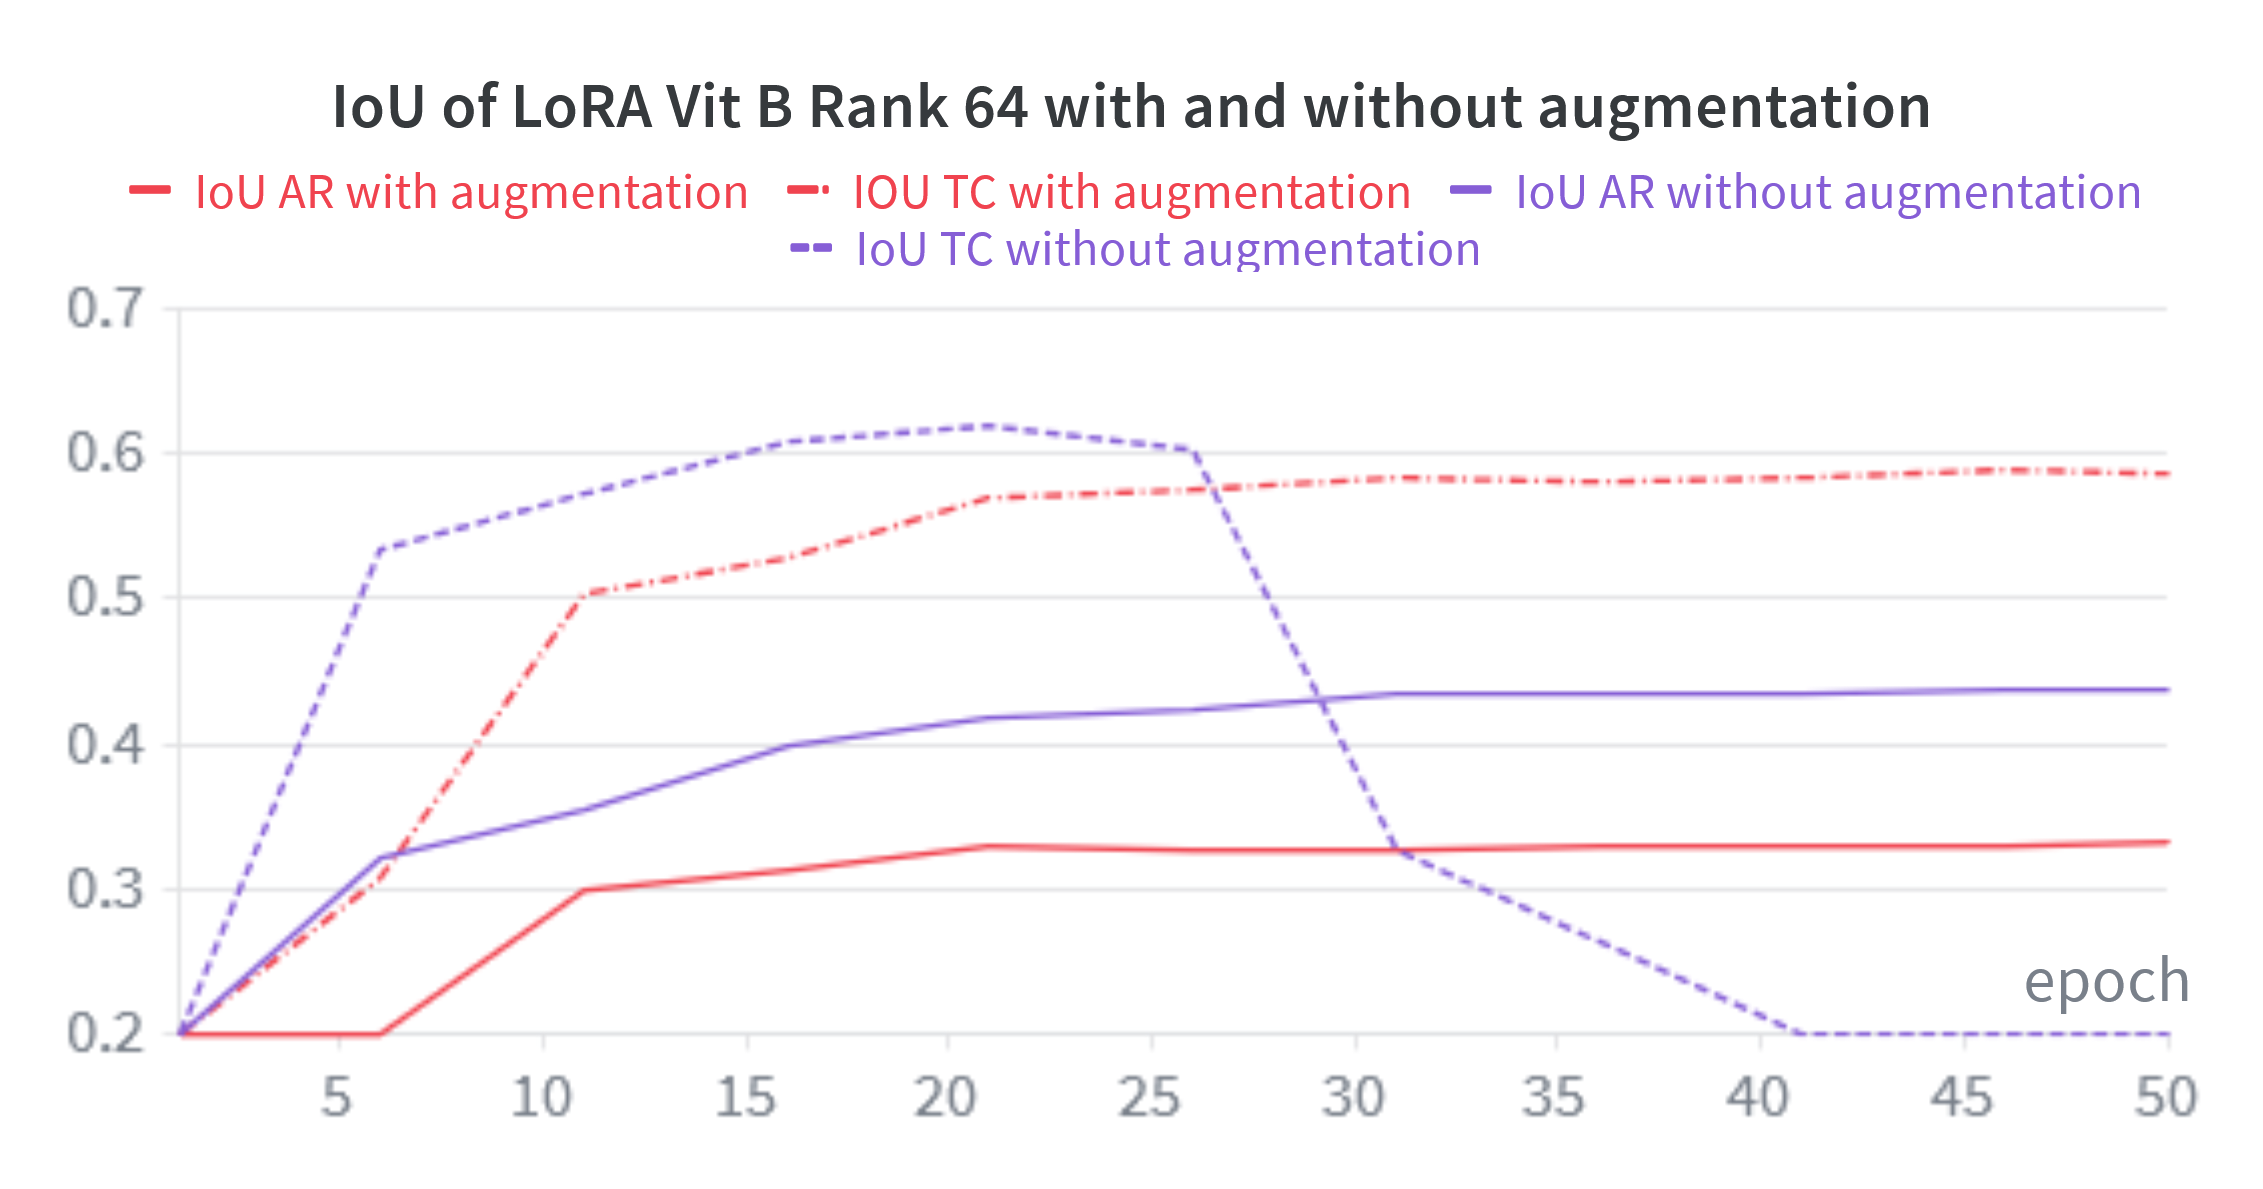
\includegraphics[width=\textwidth]{graphics/result/lora_augmentation.png}
        \caption{Augmentation Performance}
    \end{minipage}
    \caption{Comparison between standard LoRA and augmented training.}
    \label{fig:lora_augmentation}
\end{figure}

\subsubsection{Integrating specialized LoRA components for ARs and TCs}
